\documentclass{article}
\usepackage{arxiv}
\usepackage[utf8]{inputenc}
\usepackage[T1]{fontenc}
\usepackage{lmodern}
\usepackage{amsmath,amssymb,amsthm}
\usepackage{booktabs}
\usepackage{graphicx}
\usepackage{xcolor}
\usepackage[colorlinks=true,linkcolor=blue!50!black,citecolor=blue!50!black,urlcolor=blue!50!black]{hyperref}
\usepackage{algorithm}
\usepackage{algpseudocode}
\usepackage{caption}
\captionsetup{font=small,labelfont=bf}
\usepackage{enumitem}
\setlist{nosep,leftmargin=*}

\newtheorem{definition}{Definition}
\newtheorem{hypothesis}{Hypothesis}

\title{Learning to Work and Save in a Shared Economy:\\
Decentralized Multi-Agent Reinforcement Learning\\
versus the Known-Model Aiyagari Equilibrium}

\author{%
\textbf{Aryan Meshram} (24110054)\quad
\textbf{Chaitanya Sharma} (23110072)\\
\textbf{Pratik Kumar Dhaker} (24110277)\quad
\textbf{Saksham Chourasia} (24110312)}

\begin{document}
\maketitle

\begin{abstract}
We ask how close decentralized multi-agent reinforcement learning (MARL) gets to the exact competitive equilibrium of
a heterogeneous-agent economy. We build a vectorized Bewley--Aiyagari simulator with endogenous labour, taxes and
lump-sum rebates whose resource constraint holds to $10^{-9}$. We solve the same finite-state economy exactly with a
known-model benchmark (endogenous-grid dynamic programming, histogram distribution and a Brent market-clearing fixed
point), and train shared-policy IPPO and MAPPO households in it (49 runs over five population sizes, four observation
levels and seven tax regimes). Learners match equilibrium labour supply to within $0.003$ hours and lose only
$1.3$--$1.4\%$ of consumption-equivalent welfare, against $13.5\%$ for the best constant policy. However, they
under-accumulate capital by about $14\%$, produce too little wealth inequality (Gini $0.46$ vs.\ $0.55$), and remain
exploitable: an exact best response gains $0.4\%$, a gain that a PPO-trained deviator fails to find. The capital gap
does not shrink as $1/N$ but sits on a learning floor; observing prices reduces it, while observing aggregates does
not. Under income taxes, learners reproduce the signs and roughly the elasticities of the equilibrium capital and labour
responses, but not the distributional response.
\end{abstract}

\section{Introduction}
An economy is a large multi-agent system. Households choose how much to work and save, while aggregate choices
determine capital, labour, wages and returns; taxes and redistribution further change incentives. Traditional
macroeconomic models assume agents know the model and solve for equilibrium, whereas learning-based economic
simulators let agents adapt through interaction.

In the Bewley--Huggett--Aiyagari family~\cite{aiyagari,huggett}, households face idiosyncratic income risk, save in a
single asset and take prices as given; equilibrium is obtained through household dynamic programming and a
market-clearing fixed point. In the infinite-population limit this is a mean-field game~\cite{lasry,light}, and
reinforcement learning has been used to find regularized mean-field equilibria~\cite{xu}. Conversely, the AI
Economist~\cite{aiecon} and TaxAI~\cite{taxai} place learning agents inside economic simulators, and Curry et
al.~\cite{curry} study general equilibrium with deep RL. TaxAI in particular benchmarks MARL households and
governments in a Bewley--Aiyagari simulator with up to $10^4$ households, but it has no exact equilibrium to compare
the learned behaviour against.

Our project connects the two views. We build one finite-$N$ economy, solve it with a known-model benchmark (B1), train
decentralized MARL households in the \emph{same} environment, and measure gaps in aggregates, individual policies,
welfare, inequality and exploitability. The central question is:
\emph{how close does the learned economy get to the known-model competitive equilibrium, and how does this depend on
$N$, on the information available to households, and on the tax regime?}

\textbf{Contributions.} (i) An exactly-accounted, vectorized simulator whose resource constraint is verified to
$10^{-9}$ by an automated test; (ii) a dynamic-programming ground truth (EGM, histogram distribution, Brent fixed
point), cross-validated against value-function iteration; (iii) shared-policy IPPO and MAPPO households trained under
four observation levels, five population sizes and seven tax regimes (49 training runs); (iv) aggregate, policy,
consumption-equivalent welfare, inequality and two exploitability metrics (an exact DP best response and a PPO best
response); (v) quantitative tests of four hypotheses H1--H4. All numbers below are produced by the code in our
repository (Section~\ref{sec:repo}).

\section{Preliminaries and Problem Formulation}
Let $\mathcal N=\{1,\dots,N\}$ index households and $t=0,1,\dots$ periods. Household $i$ has assets $a_i^t\ge0$,
productivity $e_i^t>0$, saving ratio $p_i^t\in[p_{\min},p_{\max}]\subset(0,1)$ and hours
$h_i^t=h_{\min}+(h_{\max}-h_{\min})\hat h_i^t$, $\hat h_i^t\in[0,1]$. Aggregates are capital $K_t$, effective labour
$L_t$, output $Y_t$ and $\kappa_t=K_t/L_t$; prices are $W_t,R_t$ and $r_t=R_t-\delta$.

\begin{definition}[Markov game]
$(\mathcal N,\mathcal S,\{\mathcal O_i\},\{\mathcal A_i\},P,\{R_i\},\beta)$ with state space, observations, actions,
transition kernel, rewards and discount factor; it is general-sum when rewards need not sum to a constant.
\end{definition}
\begin{definition}[Competitive prices]
With $Y=K^\alpha L^{1-\alpha}$: $W=(1-\alpha)\kappa^\alpha$, $R=\alpha\kappa^{\alpha-1}$, $\kappa=K/L$.
\end{definition}
\begin{definition}[HSV tax~\cite{hsv}]
$\mathcal T(x)=x-(1-\tau)x^{1-\xi}/(1-\xi)$; $\xi=0$ gives the proportional tax $\tau x$ (used in all experiments).
\end{definition}

\textbf{Dynamics.} $\log e_i^{t+1}=\rho_e\log e_i^t+\sigma_e u_i^{t+1}$, discretized with a 7-state Rouwenhorst
chain~\cite{rouwen} that is used \emph{both} by the simulator and by B1, so B1 is the exact equilibrium of the
simulated economy (levels normalised to $\mathbb E[e]=1$). Households observe $o_i^t$ and simultaneously choose
$(p_i^t,\hat h_i^t)$. Then
\begin{gather*}
L_t=\max\big(\textstyle\sum_i e_i^th_i^t,\,L_{\min}\big),\quad \kappa_t=\mathrm{clip}(K_t/L_t,\kappa_{\min},\kappa_{\max}),\quad
K_t=\textstyle\sum_i a_i^t,\\
y_i^t=W_te_i^th_i^t+r_ta_i^t,\quad S_t=\textstyle\sum_i[\mathcal T(y_i^t)+\mathcal T^a(a_i^t)],\quad \nu_t=\psi S_t/N,\quad G_t=(1-\psi)S_t,\\
m_i^t=a_i^t+y_i^t-\mathcal T(y_i^t)-\mathcal T^a(a_i^t)+\nu_t,\quad a_i^{t+1}=p_i^tm_i^t,\quad c_i^t=(1-p_i^t)m_i^t,\\
R_i^t=u(c_i^t,h_i^t)=\frac{(c_i^t)^{1-\theta}}{1-\theta}-\chi\frac{(h_i^t)^{1+\varphi}}{1+\varphi}.
\end{gather*}
Because production is constant-returns, $W_tL_t+R_tK_t=Y_t$, and summing budgets gives
$Y_t=C_t+K_{t+1}-(1-\delta)K_t+G_t$ whenever no safeguard binds. Every household maximizes
$J_i=\mathbb E\sum_t\beta^tR_i^t$; with one shared policy $\pi_\vartheta$ the learning objective is
$\bar J(\vartheta)=\frac1N\sum_iJ_i(\pi_\vartheta,\dots,\pi_\vartheta)$.

\textbf{Benchmark B1.} Given $(\kappa,\nu)$ a price-taking household solves
$V(a,e)=\max_{a'\ge0,\,h\in[h_{\min},h_{\max}]}\{u(m(a,e,h)-a',h)+\beta\mathbb E[V(a',e')\mid e]\}$. With stationary
distribution $\mu_{\kappa,\nu}$, $K^s=\int a\,d\mu$, $L^s=\int eh^\star d\mu$, and $(\kappa^\star,\nu^\star)$ solves
$K^s/L^s=\kappa^\star$, $\nu^\star=\psi\int[\mathcal T(y)+\mathcal T^a(a)]d\mu$. As $N\to\infty$ an individual's
price impact vanishes, which is why B1 is the natural mean-field reference~\cite{lasry,xu}.

\textbf{Observation levels.} O0: $(a_i,e_i)$; O1: O0 + lagged prices $(W_{t-1},r_{t-1})$; O2: O1 + $K_t/N$, $L_{t-1}/N$;
O3: O2 + TaxAI-style wealth-group statistics (mean wealth, lagged income and productivity of the top-10\% and
bottom-50\%)~\cite{taxai}.

\textbf{Hypotheses.}
\textbf{H1} (equilibrium recovery): MARL approaches B1 in aggregates but may differ in the tails of the wealth distribution.
\textbf{H2} (population size): price impact is $O(1/N)$, so the gap behaves as $\Delta(N)\approx cN^{-1}+\Delta_0$ with a learning-noise floor $\Delta_0$.
\textbf{H3} (information): moving from O0 to O2 substantially reduces gaps; O3 adds less.
\textbf{H4} (tax response): MARL and B1 predict the same signs of labour and capital responses to the net-of-tax rate, possibly with different magnitudes.

\section{Methodology}\label{sec:method}
The system has six components (C1--C6), each a module of the repository.

\subsection{C1: Vectorized simulator with exact accounting}
The economy is simulated as $M$ independent economies of $N$ households held in $[M,N]$ \texttt{float64} PyTorch
tensors, so one call advances all households of all economies by one period in the order of
Section~2. Actions are normalised to $[0,1]^2$ and mapped to $p\in[0.001,0.99]$ and $h\in[0,1]$. Safeguards:
$L_{\min}=10^{-3}N$, $\kappa\in[0.5,60]$, and a consumption floor $c\ge10^{-3}$ used \emph{only} inside the utility
(never in the budget), so accounting stays exact. An automated test (\texttt{tests/test\_accounting.py}) simulates 16
economies for 50 periods under random actions for 8 configurations ($N\in\{10,100\}$, four
$(\tau,\tau^a,\psi,\xi)$ settings including a progressive schedule) and asserts
$|Y_t-C_t-K_{t+1}+(1-\delta)K_t-G_t|/Y_t<10^{-9}$ at every non-safeguarded step; it also checks
$a'+c=m$, $N\nu+G=S$, and $WL+RK=Y$.

\textbf{Calibration.} $\alpha=0.36$, $\delta=0.06$, $\beta=0.96$, $\theta=1.5$, $\varphi=2$, $\rho_e=0.9$,
$\sigma_e=0.2$. $\chi=29.70$ is chosen by Brent's method so that mean hours in the $\tau=0$ B1 equilibrium equal
$h_{\max}/3$, and initial wealth is lognormal with $\sigma_a=1.8$ and mean equal to B1 capital per household
($2.953$) (\texttt{scripts/calibrate.py}).

\subsection{C2: Known-model benchmark B1}
Algorithm~\ref{alg:b1} computes the stationary recursive competitive equilibrium. The household problem is solved
with the endogenous grid method (EGM)~\cite{egm} extended to endogenous labour: on a 200-point power-spaced grid
of next-period assets $a'\in[0,400]$, the Euler equation gives consumption, the intratemporal condition
$\chi h^{\varphi}=c^{-\theta}(1-\tau)We$ gives hours, and the budget inverts to current assets. Below the
endogenous grid's first point the borrowing constraint binds; there $a'=0$ and $h$ solves
$\chi h^\varphi=(R_aa+w_eh+\nu)^{-\theta}w_e$ by bisection ($R_a=1+(1-\tau)r-\tau^a$, $w_e=(1-\tau)We$). The
stationary distribution uses Young's histogram method~\cite{young} on a 1000-point grid (sparse transition matrix,
power iteration to $10^{-13}$), and $\kappa^\star$ is found by Brent's method on $K^s/L^s-\kappa$ inside the bracket
$r\in[0,\,((1/\beta-1)+\tau^a)/(1-\tau))$ with a damped fixed point for $\nu^\star$ at each $\kappa$.
\emph{Validation:} market clearing holds to $10^{-6}$; mean (max) $\log_{10}$ Euler-equation errors are
$-7.28$ ($-4.10$) at $\tau=0$, the worst of the seven tax regimes (best: $-7.56$ ($-5.04$))%
; and a brute-force value-function iteration on a separate grid reproduces the EGM saving and
hours policies to within grid resolution (\texttt{tests/test\_b1.py}, 6 tests).

\begin{algorithm}[t]
\caption{B1: stationary equilibrium with endogenous labour (EGM + histogram + Brent)}\label{alg:b1}
\small
\begin{algorithmic}[1]
\Function{Household}{$W,r,\nu$} \Comment{EGM; $c_0$ = constrained guess}
\Repeat
  \State $\tilde c(a'_j,e)\gets\big(\beta R_a\sum_{e'}P(e'|e)\,c(a'_j,e')^{-\theta}\big)^{-1/\theta}$;\;
  $\tilde h\gets\mathrm{clip}\big((\tilde c^{-\theta}w_e/\chi)^{1/\varphi}\big)$
  \State $\tilde a\gets(\tilde c+a'_j-w_e\tilde h-\nu)/R_a$;\; $c(a,e)\gets$ interpolate $(\tilde a,\tilde c)$; constrained FOC for $a<\tilde a_0$
\Until{$\max|c^{new}-c|/(1+c)<10^{-10}$}
\EndFunction
\Function{Excess}{$\kappa$}
  \State $W,r\gets$ prices$(\kappa)$;\; $\nu\gets0$
  \Repeat\; policy $\gets$\Call{Household}{$W,r,\nu$};\; $\mu\gets$ Young histogram fixed point;\; $\nu\gets\frac12\nu+\frac12\psi S(\mu)$
  \Until{$|\Delta\nu|<10^{-11}$}
  \State \Return $K^s(\mu)/L^s(\mu)-\kappa$
\EndFunction
\State $\kappa^\star\gets$ Brent root of \Call{Excess}{$\cdot$};\; \Return policy, $\mu^\star$, $(\kappa^\star,\nu^\star)$
\end{algorithmic}
\end{algorithm}

\subsection{C3: Baselines}
\textbf{B1-in-simulator:} the DP policy is executed by all $N$ households in the finite-$N$ simulator. A household
in state $(a,e)$ plays $p=a'(a,e)/m^\star(a,e)$ and $h=h(a,e)$, where $m^\star$ is cash-on-hand at equilibrium
prices, so B1 and MARL are compared under identical dynamics, safeguards and random numbers.
\textbf{B0:} the $\tau=0$ economy, the reference for tax responses in E4 (in E1, where $\tau=0$, B0 and B1 coincide).
\textbf{B2:} the best constant policy $(\bar p,\bar h)$ shared by everyone, found by a $19\times15$ grid search in
the simulator followed by an $11\times11$ refinement. \textbf{Random:} uniform actions.

\subsection{C4: Shared-policy IPPO and MAPPO}
All households share one actor (parameter sharing) but each maximizes its \emph{own} discounted utility, so the game
stays general-sum. The actor is a 2$\times$64 tanh MLP that outputs the concentrations $1+\mathrm{softplus}(\cdot)$ of
two independent Beta distributions over $(\hat p,\hat h)\in(0,1)^2$; Beta policies respect the action bounds without
clipping bias. IPPO~\cite{ippo} uses a local critic $V(o_i)$; MAPPO~\cite{mappo} uses a centralized critic
$V(o_i,g(s))$ where $g$ is a permutation-invariant 11-dimensional summary of the whole economy (mean wealth,
5 wealth quantiles, dispersion, mean productivity, lagged prices and labour). Training follows PPO~\cite{ppo}
with GAE~\cite{gae} (Algorithm~\ref{alg:ppo}). The RL discount equals the household discount $\beta$, so the RL objective
\emph{is} the household's objective; episodes last 200 periods from a fresh lognormal draw and are bootstrapped with
$V(s_{200})$ because the economic problem has an infinite horizon. Rewards are scaled by $1-\beta$. Each iteration
collects $8\times10^4$ household-steps ($M=8\times10^4/(200N)$ economies; for $N=1000$, $M=1$ gives $2\times10^5$),
followed by 4 epochs of minibatch (8192) Adam updates; learning rate $10^{-3}$ linearly decayed to 0 over 300
iterations, clip $0.2$, $\lambda=0.95$, entropy $10^{-3}$, value coefficient $0.5$, gradient-norm clip $0.5$.
The learning rate was selected from $\{3\cdot10^{-4},10^{-3}\}$ on a single tuning seed.

\begin{algorithm}[t]
\caption{Shared-policy IPPO / MAPPO for $N$ households}\label{alg:ppo}
\small
\begin{algorithmic}[1]
\For{iteration $k=1,\dots,300$}
  \State reset $M$ economies with lognormal wealth and stationary productivity
  \For{$t=0,\dots,199$} \Comment{all $M\cdot N$ households act in parallel}
    \State $o_i^t\gets$ \Call{Obs}{$s^t$, level}; sample $(\hat p_i^t,\hat h_i^t)\sim\mathrm{Beta}(\pi_\vartheta(o_i^t))$; step simulator; store $(o_i^t,a_i^t,R_i^t,\log\pi)$
  \EndFor
  \State critic input $x_i^t=o_i^t$ (IPPO) or $[o_i^t,g(s^t)]$ (MAPPO); per-household GAE with $\gamma=\beta$, bootstrap at $t=200$
  \State 4 epochs of clipped-surrogate + value + entropy loss on minibatches pooled over households
\EndFor
\end{algorithmic}
\end{algorithm}

\subsection{C5: Evaluation metrics}
Policies are evaluated deterministically (Beta mean) in 8 economies for 500 periods from a common lognormal draw with
\emph{common random numbers} across all policies. Stationary statistics are averaged over $t\in[300,500)$.
\textbf{Aggregate gap:} $|\kappa^{\rm MARL}-\kappa^\star|/\kappa^\star$, plus hours and saving-rate ($\sum a'/\sum m$) gaps.
\textbf{Policy gap:} $\sum_{a,e}\mu^\star(a,e)\,|p^{\rm MARL}(a,e)-p^{\rm B1}(a,e)|$ and likewise for $h$, with the
learner's aggregate inputs fixed at their long-run averages.
\textbf{Welfare:} $\bar J$ is the average discounted utility over the 500 periods. The consumption-equivalent
\emph{welfare loss} $\lambda$ of a policy relative to B1-in-simulator solves
$(1+\lambda)^{1-\theta}U_c-U_h=\bar J^{\rm B1}$, with $U_c,U_h$ the consumption and labour parts of its welfare
(closed form).
\textbf{Inequality:} wealth Gini and top-10\% share. \textbf{Convergence:} the first evaluation (every 20 iterations)
at which $\bar J$ closes 95\% of its total improvement. \textbf{Seeds:} 5 for E1, 3 for E2--E4 (mean $\pm$ s.d.).

\subsection{C6: Approximate exploitability}
We freeze the learned population and ask how much one household gains by deviating. (a)~\textbf{DP best response:}
B1's household solver is run at the learned economy's long-run prices $(\bar W,\bar r,\bar\nu)$, which is the exact
best response of a price-taker. If under-saving pushes $\beta R_a\ge1$, no stationary optimum exists, and we use the
period-0 policy of the 200-period problem (200 backward EGM steps), which is still a valid deviation. (b)~\textbf{PPO best response:} a single deviator, warm-started from the shared actor
with a fresh critic, is trained for 100 iterations in 128 economies while everyone else plays the frozen policy;
checkpoints are selected on a validation snapshot. Both deviations are tested in the simulator from a stationary
snapshot of the learned economy (32 economies), placing the deviator at the 10th, 50th and 90th wealth percentiles
with median productivity, over 200 periods with common random numbers. Exploitability is the deviator's
consumption-equivalent gain in \%; any positive value means the learned profile is not a Nash equilibrium.

\section{Results}\label{sec:results}
Unless stated otherwise, the setting is $N=100$, observation level O3, $\tau=0$ and $\psi=1$ (B0 $=$ B1). Each IPPO run takes
about 10 minutes on 2 CPU threads ($2.4\times10^7$ household-steps). Numbers are mean $\pm$ s.d.\ across seeds, and every
entry is produced by \texttt{scripts/make\_report\_assets.py}.

\subsection{E1: Does decentralized learning recover the competitive equilibrium?}
\begin{table}[t]
\centering\small
\caption{E1 at $N=100$. B1-in-simulator executes the DP policy in the same finite-$N$ simulator with common random
numbers. W-loss: consumption-equivalent welfare loss relative to B1-in-simulator. DP-BR / PPO-BR: a single deviator's
consumption-equivalent gain (mean of the 10th, 50th and 90th wealth percentiles).}\label{tab:e1}
\resizebox{\linewidth}{!}{\begin{tabular}{lccccccccc}
\toprule
Policy & $\kappa$ & $K/N$ & hours & $a'/m$ & Gini & Top-10\% & W-loss (\%) & DP-BR (\%) & PPO-BR (\%)\\
\midrule
B1 (theory, $N{=}\infty$) & 8.713 & 2.953 & 0.333 & 0.840 & 0.549 & 0.342 & -- & -- & --\\
B1 in simulator & 8.745 & 2.955 & 0.333 & 0.840 & 0.545 & 0.337 & 0.00 & -0.01 & --\\
B2 (best constant) & 7.985 & 2.790 & 0.350 & 0.830 & 0.196 & 0.174 & 13.53 & 3.32 & --\\
Random & 0.889 & 0.442 & 0.500 & 0.495 & 0.513 & 0.352 & 3583.29 & -- & --\\
IPPO ($n{=}5$) & 7.532 $\pm$ 0.086 & 2.520 $\pm$ 0.032 & 0.334 $\pm$ 0.002 & 0.823 $\pm$ 0.001 & 0.464 $\pm$ 0.017 & 0.297 $\pm$ 0.007 & 1.36 $\pm$ 0.10 & 0.40 $\pm$ 0.07 & -0.00 $\pm$ 0.00\\
MAPPO ($n{=}5$) & 7.563 $\pm$ 0.122 & 2.530 $\pm$ 0.052 & 0.334 $\pm$ 0.002 & 0.824 $\pm$ 0.002 & 0.454 $\pm$ 0.010 & 0.291 $\pm$ 0.010 & 1.30 $\pm$ 0.19 & 0.42 $\pm$ 0.13 & 0.02 $\pm$ 0.05\\
\bottomrule
\end{tabular}
}
\end{table}
\begin{figure}[t]
\centering
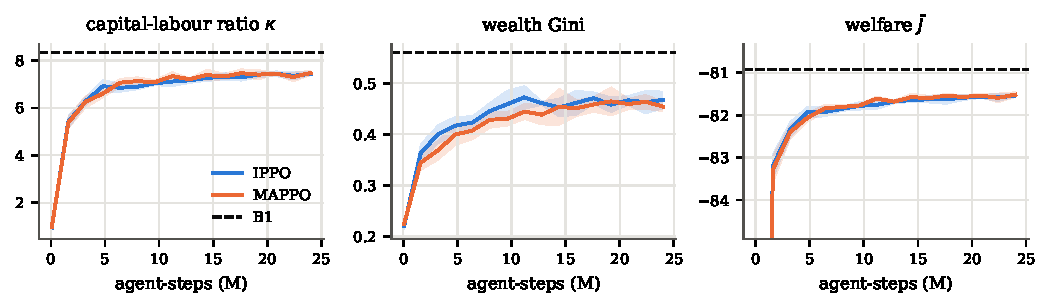
\includegraphics[width=\linewidth]{figures/fig_e1_learning.pdf}
\caption{E1 learning curves (5 seeds, mean $\pm$ s.d.), evaluated every 20 iterations with the deterministic
policy. Dashed: B1 executed under the same evaluation protocol.}\label{fig:e1learn}
\end{figure}
\begin{figure}[t]
\centering
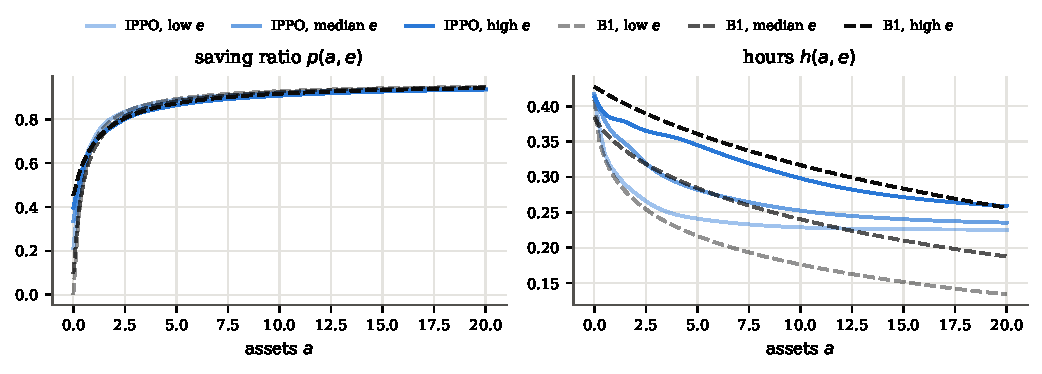
\includegraphics[width=\linewidth]{figures/fig_e1_policy.pdf}
\caption{Learned (IPPO seed 0) and B1 policy functions for low, median and high productivity, with the learner's
aggregate inputs fixed at their long-run means.}\label{fig:e1policy}
\end{figure}
\begin{figure}[t]
\centering
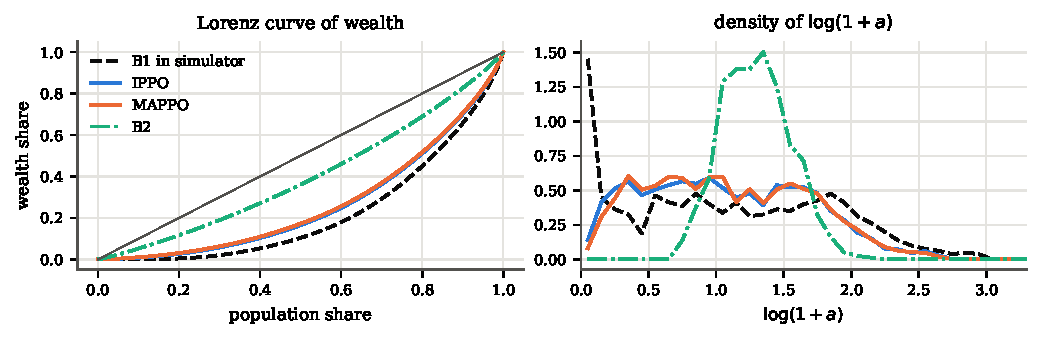
\includegraphics[width=\linewidth]{figures/fig_e1_wealth.pdf}
\caption{Stationary wealth distribution (pooled over seeds and 8 evaluation economies, $t=500$).}\label{fig:e1wealth}
\end{figure}

Table~\ref{tab:e1} and Figures~\ref{fig:e1learn}--\ref{fig:e1wealth} give the answer. \textbf{Aggregates.} Welfare
converges within 40 iterations ($3.2\times10^6$ household-steps) for both learners, while $\kappa$ keeps creeping up
slowly. The resulting stationary economy \emph{matches B1 in
labour supply exactly} (hours $0.334$ vs.\ $0.333$) but \emph{under-accumulates capital}: $\kappa=7.53\pm0.09$ (IPPO)
and $7.56\pm0.12$ (MAPPO) against $\kappa^\star=8.71$, a gap of $13.6\%$, which is about $35$ times the finite-$N$
gap of B1 itself ($0.4\%$). The interest rate is correspondingly higher ($3.9\%$ vs.\ $3.0\%$). \textbf{Policies.}
The saving-ratio function is learned closely (policy gap $0.047$; Figure~\ref{fig:e1policy}, left), and the remaining
error sits near the borrowing constraint, where poor households save too much and rich ones slightly too little. Hours
are learned less well: the learned wealth effect on labour is too weak, so wealthy low-productivity households
work $0.23$ instead of $0.14$. \textbf{Inequality.} The learned economy is markedly more equal (Gini $0.46$
vs.\ $0.55$, top-10\% share $0.30$ vs.\ $0.34$): it lacks both the mass of constrained households at $a=0$ and the
right tail (Figure~\ref{fig:e1wealth}). \textbf{Welfare.} The consumption-equivalent loss is only $1.36\pm0.10\%$
(IPPO) and $1.30\pm0.19\%$ (MAPPO). The best constant policy B2 loses $13.5\%$, so learning closes about $90\%$ of the
welfare gap between a naive rule and the equilibrium.

\textbf{Exploitability.} The learned profile is \emph{not} a Nash equilibrium. The exact DP best response to the
learned economy's prices gains $0.40\pm0.07\%$ consumption-equivalent (10th/50th/90th percentile: $0.42/0.26/0.53\%$).
As a sanity check, the same procedure gives $-0.01\%$ against B1 and $3.3\%$ against B2. By contrast, the PPO best
response (100 iterations, warm-started) finds essentially \emph{no} improvement ($0.00\%$ IPPO, $0.02\pm0.05\%$ MAPPO).
In 9 of 10 runs no checkpoint beats the warm-start policy on the validation snapshot. A model-free deviator thus misses
the gain that the model-based deviator finds, so learning-based exploitability estimates can badly understate the
distance to equilibrium.
\textbf{MAPPO vs.\ IPPO.} The centralized critic changes nothing measurable: every metric overlaps within one s.d.
This is consistent with the price-taking structure: with $N=100$ a household's value depends on the economy only
through two prices, which O3 already summarises.
\emph{Verdict on H1: supported.} MARL approaches B1 in labour supply and welfare, deviates by 14\% in capital,
and deviates most in the tails of the wealth distribution.

\subsection{E2: Does the gap shrink with population size?}
\begin{table}[t]
\centering\small
\caption{E2: population size (IPPO, O3). B1-sim gap: $|\kappa^{\rm B1\text{-}sim}-\kappa^\star|/\kappa^\star$, i.e.\ the
finite-$N$ error of the exact policy itself. Household-steps per run: $2.4\times10^7$ ($N\le100$), $1.8\times10^7$
($N=300$, one economy per iteration), $6\times10^7$ ($N=1000$).}\label{tab:e2}
\resizebox{\linewidth}{!}{\begin{tabular}{rcccccccc}
\toprule
$N$ & $n$ & $|\Delta\kappa|/\kappa^\star$ & B1-sim gap & $p$-gap & $h$-gap & W-loss (\%) & DP-BR (\%) & time (min)\\
\midrule
10 & 3 & 0.155 $\pm$ 0.008 & 0.023 & 0.065 $\pm$ 0.006 & 0.022 $\pm$ 0.003 & -1.54 $\pm$ 0.05 & -0.33 $\pm$ 0.04 & 7.6\\
30 & 3 & 0.154 $\pm$ 0.018 & 0.054 & 0.056 $\pm$ 0.005 & 0.016 $\pm$ 0.001 & 0.78 $\pm$ 0.13 & 0.86 $\pm$ 0.24 & 9.2\\
100 & 5 & 0.136 $\pm$ 0.010 & 0.004 & 0.047 $\pm$ 0.010 & 0.014 $\pm$ 0.001 & 1.36 $\pm$ 0.10 & 0.40 $\pm$ 0.07 & 9.8\\
300 & 3 & 0.156 $\pm$ 0.027 & 0.003 & 0.062 $\pm$ 0.011 & 0.019 $\pm$ 0.001 & 2.52 $\pm$ 0.29 & 1.08 $\pm$ 0.37 & 8.9\\
1000 & 3 & 0.088 $\pm$ 0.007 & 0.005 & 0.038 $\pm$ 0.008 & 0.012 $\pm$ 0.002 & 1.47 $\pm$ 0.03 & 0.18 $\pm$ 0.03 & 22.6\\
\bottomrule
\end{tabular}
}
\end{table}
\begin{figure}[t]
\centering
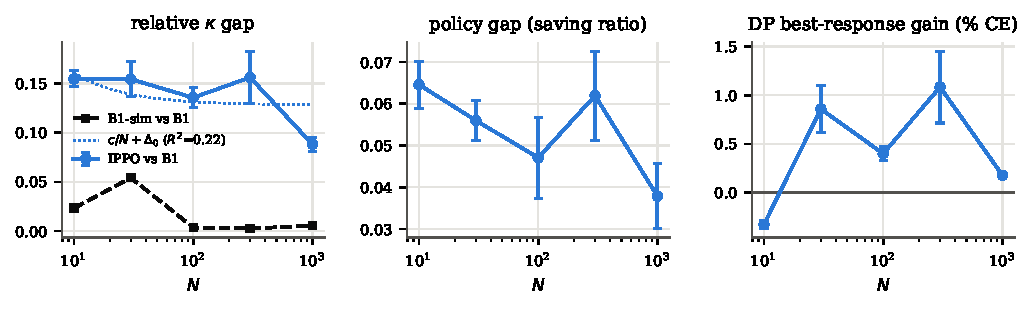
\includegraphics[width=\linewidth]{figures/fig_e2_population.pdf}
\caption{E2: capital gap with the fitted $c/N+\Delta_0$ curve, saving-policy gap and DP best-response gain versus $N$.}\label{fig:e2}
\end{figure}
H2 predicted $\Delta(N)\approx c/N+\Delta_0$. The data (Table~\ref{tab:e2}, Figure~\ref{fig:e2}) show that the
\emph{learning floor dominates}. The capital gap is $15.5\%$, $15.4\%$, $13.6\%$ and $15.6\%$ for
$N=10,30,100,300$, and $8.8\%$ for $N=1000$. The fit gives $\Delta_0=12.8\%$ with $R^2=0.22$ (a $c/\sqrt N$ fit does
no better, $R^2=0.33$). The gap is in fact ordered by the \emph{sample budget} rather than by $N$: the worst run
($N=300$) has the fewest household-steps and the best ($N=1000$) the most, so the $N=1000$ improvement cannot be
attributed to vanishing price impact. Price impact itself is visible only at the smallest $N$. At $N=10$, B1 executed
in the simulator \emph{loses} welfare relative to the learners (W-loss $-1.54\%$), and the DP best response computed at
mean prices is a \emph{worse} deviation ($-0.33\%$). With ten households prices fluctuate strongly (the s.d.\ of $\kappa$
across economies is $1.2$ under B1, against $0.16$ at $N=100$). A price-taking policy that ignores this volatility is
then no longer optimal, while learners adapt to the actual dynamics. For $N\ge30$ the known-model reference is the
better policy again. \emph{Verdict on H2: not supported at our training budget.} An $O(1/N)$ effect exists in the
benchmark itself (B1-sim gap) but is swamped by a ${\approx}13\%$ learning floor in MARL.


\subsection{E3: Does information help?}
\begin{table}[t]
\centering\small
\caption{E3: observation levels (IPPO, $N=100$). conv.\ iter: first evaluation reaching 95\% of the final welfare
improvement.}\label{tab:e3}
\begin{tabular}{lccccccc}
\toprule
Obs. & $n$ & $|\Delta\kappa|/\kappa^\star$ & $p$-gap & $h$-gap & W-loss (\%) & DP-BR (\%) & conv. iter\\
\midrule
O0 & 3 & 0.184 $\pm$ 0.002 & 0.044 $\pm$ 0.008 & 0.012 $\pm$ 0.001 & 1.21 $\pm$ 0.08 & 0.81 $\pm$ 0.05 & 33\\
O1 & 3 & 0.158 $\pm$ 0.016 & 0.036 $\pm$ 0.006 & 0.012 $\pm$ 0.002 & 1.27 $\pm$ 0.27 & 0.49 $\pm$ 0.17 & 27\\
O2 & 3 & 0.157 $\pm$ 0.003 & 0.037 $\pm$ 0.006 & 0.012 $\pm$ 0.000 & 1.19 $\pm$ 0.06 & 0.48 $\pm$ 0.05 & 33\\
O3 & 5 & 0.136 $\pm$ 0.010 & 0.047 $\pm$ 0.010 & 0.014 $\pm$ 0.001 & 1.36 $\pm$ 0.10 & 0.40 $\pm$ 0.07 & 40\\
\bottomrule
\end{tabular}

\end{table}
Table~\ref{tab:e3} shows that information matters for \emph{aggregates and exploitability} but
not for welfare. Adding lagged prices (O0$\to$O1) cuts the capital gap from $18.4\%$ to $15.8\%$ and the DP best-response
gain from $0.81\%$ to $0.49\%$. Without prices a household cannot condition on the return to saving, so it
under-reacts to it. Aggregate capital and labour (O2) add nothing beyond prices, which is expected because in a
competitive economy prices are sufficient statistics for aggregates. The TaxAI group statistics (O3) reduce the gap
further to $13.6\%$ and the exploitability to $0.40\%$. The welfare loss is flat at $1.2$--$1.4\%$ across all levels,
so most of the welfare comes from the individual state $(a,e)$, which every level observes. All levels converge within
about 40 iterations. \emph{Verdict on H3: partially supported.} Prices (O1) help as predicted, but O2 adds nothing
while O3 still helps, the opposite of the predicted ordering.

\subsection{E4: Do learners respond to taxes like the equilibrium?}
\begin{table}[t]
\centering\small
\caption{E4: proportional income tax $\tau$ with revenue wasted ($\psi=0$) or rebated lump-sum ($\psi=1$). IPPO, O3,
3 seeds. B1 columns are the exact stationary equilibrium.}\label{tab:e4}
\resizebox{\linewidth}{!}{\begin{tabular}{ccccccccc}
\toprule
$\tau$ & $\psi$ & $K/N$ MARL & $K/N$ B1 & hours MARL & hours B1 & Gini MARL & Gini B1 & $\bar J$ MARL / B1\\
\midrule
0.1 & 0 & 2.327 $\pm$ 0.012 & 2.798 & 0.336 $\pm$ 0.002 & 0.338 & 0.454 & 0.538 & -85.8 / -85.3\\
0.2 & 0 & 2.193 $\pm$ 0.048 & 2.620 & 0.342 $\pm$ 0.001 & 0.342 & 0.468 & 0.531 & -90.6 / -89.9\\
0.3 & 0 & 1.985 $\pm$ 0.034 & 2.417 & 0.351 $\pm$ 0.001 & 0.348 & 0.477 & 0.523 & -96.3 / -95.5\\
0.0 & 1 & 2.520 $\pm$ 0.032 & 2.953 & 0.334 $\pm$ 0.002 & 0.333 & 0.464 & 0.545 & -81.8 / -81.3\\
0.1 & 1 & 2.218 $\pm$ 0.048 & 2.632 & 0.320 $\pm$ 0.002 & 0.321 & 0.460 & 0.551 & -81.2 / -80.6\\
0.2 & 1 & 1.943 $\pm$ 0.015 & 2.306 & 0.307 $\pm$ 0.001 & 0.307 & 0.481 & 0.556 & -80.8 / -80.1\\
0.3 & 1 & 1.650 $\pm$ 0.029 & 1.976 & 0.291 $\pm$ 0.000 & 0.294 & 0.473 & 0.563 & -80.9 / -80.0\\
\bottomrule
\end{tabular}
}
\end{table}
\begin{figure}[t]
\centering
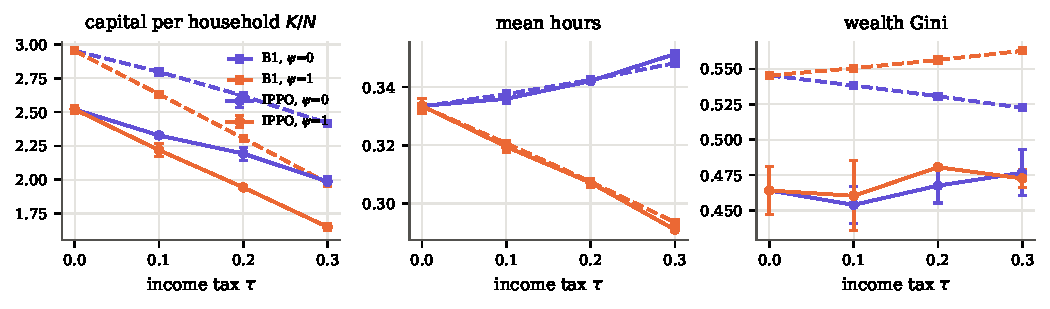
\includegraphics[width=\linewidth]{figures/fig_e4_tax.pdf}
\caption{E4: capital, hours and wealth Gini versus $\tau$. Solid: IPPO (mean $\pm$ s.d.); dashed: B1 equilibrium.}\label{fig:e4}
\end{figure}
The tax experiment is the strongest result (Table~\ref{tab:e4}, Figure~\ref{fig:e4}). \textbf{Signs.} MARL reproduces
every qualitative prediction of the equilibrium. Capital falls with $\tau$ in both regimes. Hours \emph{rise} with
$\tau$ when revenue is wasted, because the income effect dominates when households are poorer. Hours \emph{fall} when
revenue is rebated, because the substitution effect dominates once the rebate removes the income effect. The rebate
regime cuts capital more. \textbf{Magnitudes.} The elasticities with respect to the net-of-tax rate are close to B1's:
$\varepsilon_K=0.65$ vs.\ $0.56$ and $\varepsilon_h=-0.15$ vs.\ $-0.12$ ($\psi=0$); $\varepsilon_K=1.18$ vs.\ $1.13$
and $\varepsilon_h=0.38$ vs.\ $0.36$ ($\psi=1$). Hours match B1 to within $0.003$ in every regime. The capital shortfall is
a nearly constant \emph{level} effect: learned $\kappa$ is $83$--$86\%$ of $\kappa^\star$ in all seven regimes, so it
largely cancels in comparative statics. \textbf{Where MARL fails.} Inequality responds to taxes with the wrong
sensitivity. In B1, the rebate raises the Gini (from $0.545$ to $0.563$) because the lump sum makes low-wealth
households less willing to save, and wasted revenue lowers it. MARL's Gini stays at $0.45$--$0.48$ with no clear trend
in either regime. In $13$ of the $49$ runs (mostly $\tau\ge0.2$ and O0), under-saving pushes the after-tax return
above $1/\beta$, which is impossible in a stationary equilibrium; there we use the 200-period finite-horizon DP best
response. \emph{Verdict on H4: supported} for signs and, unexpectedly, for magnitudes of aggregate responses; not
supported for distributional responses.


\section{Discussion and Conclusion}
\textbf{Summary.} Placing MARL households and an exact equilibrium solver in the \emph{same} finite-$N$ economy turns
qualitative claims of the form ``learners behave like an economy'' into measured gaps. Shared-policy PPO learns the
intensive margins well: hours, the saving ratio away from the constraint, and the responses to taxes. Welfare comes
within $1.4\%$ of equilibrium. Two things are systematically missed: precautionary wealth accumulation (a
${\approx}14\%$ capital shortfall that persists across $N$, observation levels and tax regimes) and the shape of the
wealth distribution (too few constrained households, too thin a right tail). We conjecture that both stem from the long-horizon
credit-assignment problem. The benefit of an extra unit of saving arrives decades later and only in rare bad states,
so it is weak in a 200-step, $\gamma=0.96$ return and easy for a smooth stochastic policy to under-fit. This is also why
model-free exploitability (PPO-BR $\approx0$) underestimates the model-based one (DP-BR $0.4\%$).

\textbf{Hypotheses.} H1 supported; H2 not supported at our budget (learning floor ${\approx}13\%$ dominates the
$O(1/N)$ term); H3 partially (prices help, aggregates do not); H4 supported for aggregate signs and magnitudes, not for
inequality.

\textbf{Limitations.} (i) Training budget: a single learning rate was tuned on one seed and every run uses 300 iterations;
budgets differ across $N$ because economies per iteration are integers, which confounds E2. (ii) DP best responses
assume constant prices, which is inaccurate at $N=10$ and requires a finite-horizon variant when learned returns
exceed $1/\beta$. (iii) Only proportional taxes ($\xi=0$) were run, although the simulator supports HSV progressivity
and asset taxes. (iv) Evaluation starts every economy from the same lognormal draw, and stationary statistics use 200
periods after a 300-period burn-in.

\textbf{Future work.} Longer training or curricula on the horizon to test whether the capital floor is a sample-budget
effect; recurrent policies; progressive taxation; and a learning government on top of the household equilibrium, as in
TaxAI, with B1 as a reference for the households' response.

\section{Code Availability and Reproducibility}\label{sec:repo}
All code, trained models, raw results and figure scripts are in
\url{https://github.com/AryanMeshram059/fai-group42-econ-marl}. Every number and figure in this report is
regenerated from the stored runs by \texttt{python scripts/make\_report\_assets.py}; the full pipeline is
\texttt{scripts/calibrate.py} $\rightarrow$ \texttt{run\_benchmarks.py} $\rightarrow$ \texttt{run\_experiments.py}
(49 runs, resumable) $\rightarrow$ \texttt{make\_report\_assets.py}, and \texttt{pytest tests} runs the 16 accounting
and equilibrium tests. All experiments ran on a 12-core laptop CPU (no GPU); the whole grid takes about 2.5 hours
with five parallel workers.

\section{Contribution}
Tasks follow the allocation in our project proposal; the \emph{Status} column records whether the assigned task was
delivered in the final submission.

\begin{table}[h]
\centering\small
\begin{tabular}{@{}p{3.1cm}p{9.6cm}l@{}}
\toprule
Member & Assigned task & Status\\
\midrule
Aryan Meshram & Economic environment (C1): vectorized simulator, exact accounting tests, Rouwenhorst process,
calibration of $\chi$ and initial wealth & Fulfilled\\
Chaitanya Sharma & Known-model benchmark (C2, C3): EGM household solver with endogenous labour, histogram distribution,
Brent equilibrium, VFI cross-check, baselines B0/B2/Random, sanity checks & Fulfilled\\
Pratik Kumar Dhaker & MARL (C4): shared-policy IPPO and MAPPO with Beta policies, observation levels O0--O3,
learning-rate tuning, multi-seed training of the 49-run grid & Fulfilled\\
Saksham Chourasia & Evaluation (C5, C6): aggregate/policy/welfare/inequality metrics, DP and PPO best-response
exploitability, experiments E1--E4, figures and report & Fulfilled\\
\bottomrule
\end{tabular}
\end{table}


\bibliographystyle{unsrt}
\begin{thebibliography}{99}\small\setlength{\itemsep}{0pt}
\bibitem{taxai} Q.~Mi, S.~Xia, Y.~Song, H.~Zhang, S.~Zhu, and J.~Wang. TaxAI: A dynamic economic simulator and benchmark for multi-agent reinforcement learning. In \emph{Proc. AAMAS}, 1390--1398, 2024.
\bibitem{aiyagari} S.~R.~Aiyagari. Uninsured idiosyncratic risk and aggregate saving. \emph{Quarterly Journal of Economics}, 109(3):659--684, 1994.
\bibitem{huggett} M.~Huggett. The risk-free rate in heterogeneous-agent incomplete-insurance economies. \emph{J. Economic Dynamics and Control}, 17(5--6):953--969, 1993.
\bibitem{hsv} J.~Heathcote, K.~Storesletten, and G.~L.~Violante. Optimal tax progressivity: An analytical framework. \emph{Quarterly Journal of Economics}, 132(4):1693--1754, 2017.
\bibitem{xu} R.~Xu, Y.~Min, T.~Wang, T.~Wang, M.~I.~Jordan, and Z.~Yang. Finding regularized competitive equilibria of heterogeneous agent macroeconomic models via reinforcement learning. In \emph{Proc. AISTATS}, PMLR 206, 2023.
\bibitem{lasry} J.-M.~Lasry and P.-L.~Lions. Mean field games. \emph{Japanese Journal of Mathematics}, 2(1):229--260, 2007.
\bibitem{light} B.~Light and G.~Y.~Weintraub. Mean field equilibrium: Uniqueness, existence, and comparative statics. \emph{Operations Research}, 70(1):585--605, 2022.
\bibitem{aiecon} S.~Zheng et al. The AI Economist: Taxation policy design via two-level deep multiagent reinforcement learning. \emph{Science Advances}, 8(18), 2022.
\bibitem{curry} M.~Curry, A.~Trott, S.~Phade, Y.~Bai, and S.~Zheng. Finding general equilibria in many-agent economic simulations using deep reinforcement learning. arXiv:2201.01163, 2022.
\bibitem{mappo} C.~Yu et al. The surprising effectiveness of PPO in cooperative multi-agent games. In \emph{NeurIPS}, 35, 2022.
\bibitem{ippo} C.~Schroeder de Witt et al. Is independent learning all you need in the StarCraft multi-agent challenge? arXiv:2011.09533, 2020.
\bibitem{ppo} J.~Schulman, F.~Wolski, P.~Dhariwal, A.~Radford, and O.~Klimov. Proximal policy optimization algorithms. arXiv:1707.06347, 2017.
\bibitem{rouwen} K.~A.~Kopecky and R.~M.~H.~Suen. Finite state Markov-chain approximations to highly persistent processes. \emph{Review of Economic Dynamics}, 13(3):701--714, 2010.
\bibitem{egm} C.~D.~Carroll. The method of endogenous gridpoints for solving dynamic stochastic optimization problems. \emph{Economics Letters}, 91(3):312--320, 2006.
\bibitem{young} E.~R.~Young. Solving the incomplete markets model with aggregate uncertainty using the Krusell--Smith algorithm and non-stochastic simulations. \emph{J. Economic Dynamics and Control}, 34(1):36--41, 2010.
\bibitem{gae} J.~Schulman, P.~Moritz, S.~Levine, M.~Jordan, and P.~Abbeel. High-dimensional continuous control using generalized advantage estimation. In \emph{ICLR}, 2016.
\end{thebibliography}
\end{document}
